\subsection{Developers using AdaptUI}
\label{sec:developers}

Before introducing the results obtained from working with potential final users
of AdaptUI (as consumers of adapted user interfaces), an experiment has been
carried out involving developers with previous experience with Android development.
This experiment aims to evaluate the provided \acp{api} and to compare the 
differences between performing a configuration of the user interface in Android
and in AdaptUI. 

As AdaptUI provides two different \acp{api}, this experiment has been divided
in two parts. The first one deals with the adaptation \ac{api}. This \ac{api}
eases the adaptation process by calling several methods related to the aspect of 
the different elements displayed on the screen. Section~\ref{sec:adaptation_api} 
details its most significant methods. The second part's goal is to show developers 
how to modify the knowledge of the AdaptUIOnt ontology. These methods are
listed in Section~\ref{sec:knowledge_api}.

\subsubsection{The adaptation \ac{api}}
\label{sec:adaptation_api}

The adaptation \ac{api} provides a set of methods with the purpose of easing the 
adaptation process for developers. As previous Android development experience
is needed, the idea of this \ac{api} is to maintain the design paradigm established
by Android. This includes layout configuration \ac{xml} file, in which the 
declaration of the user interface elements have to be detailed; and also a
search and a declaration of the same items in the \textit{onCreate} main method
if any actions are planned with these items (e.g., change their behaviour or
colour).

The developers participating in this experiment are guided through a brief 
explanation of the available adaptation \ac{api} methods. The purpose of this
part of the experiment is to check their feedback when dealing with the AdaptUI
framework, collecting their opinions. In the experiment, a pre-defined application
with its user interface is presented. Listing~\ref{lst:default_layout} shows the 
pre-defined Android \ac{xml} layout, including a grid layout, an edit text, a 
button and a text view. The resulting user interface is shown in Figure~\ref{fig:default_layout}.

\inputminted[linenos=true, fontsize=\footnotesize, frame=lines]{xml}{5_experiments_and_results/default_layout.xml}
\captionof{listing}{The default layout defining a grid layout, a text view,
a button and an edit text.\label{lst:default_layout}}

\begin{figure}
\centering
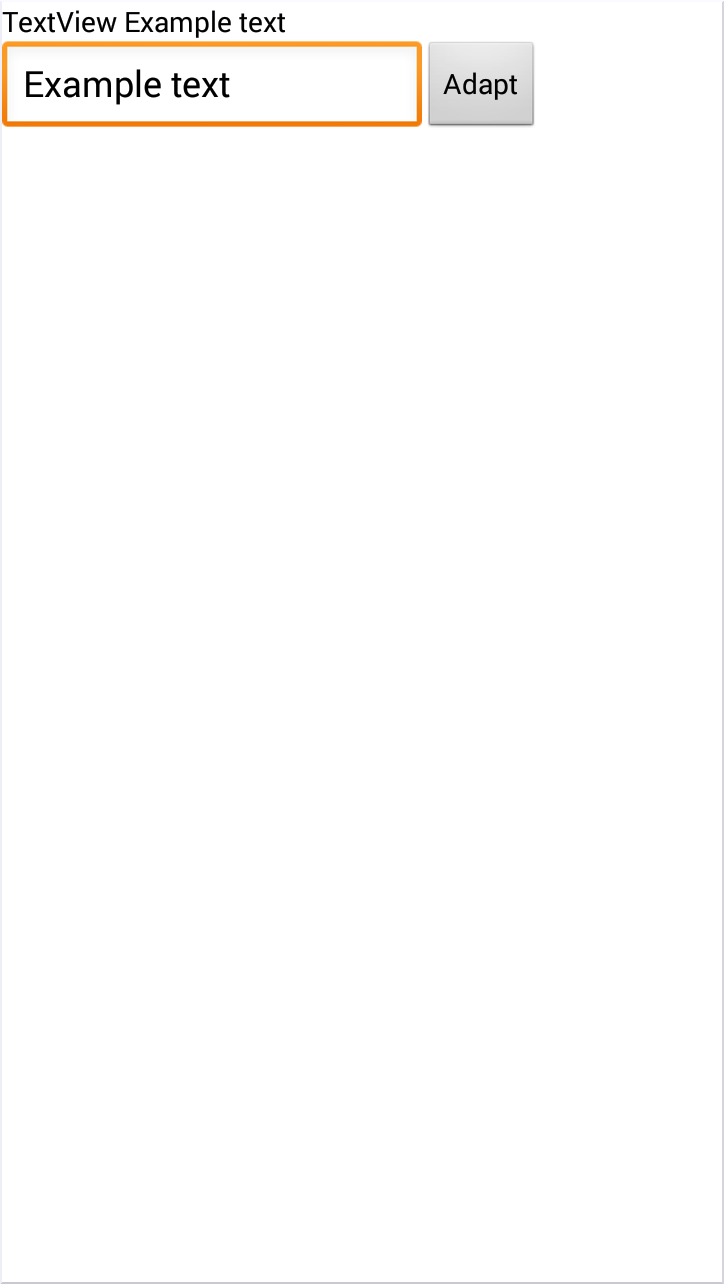
\includegraphics[width=0.25\textwidth]{default_layout.png}
\caption{The corresponding user interface considering the layout specified in
Listing~\ref{lst:default_layout}.}
\label{fig:default_layout}
\end{figure}

The usual Android code for managing the user interface is shown in Listing~\ref{lst:default_oncreate}.
Once the AdaptUI available adaptation methods are explained to the developers,
they are asked to make the mentioned user interface items dynamically adaptive.
The developers are asked to install the Capabilities Collector in their Android
devices. Then, they run it and they adapt the user interface as needed. After
the adaptation process (as users) they are asked to develop their own application,
showing a text view, an edit text, and a button. 

An example is shown in Listing~\ref{lst:adaptui_oncreate}. In it, it is shown 
how declaring an \textit{AdaptUI} object the adaptation of the views is easy and 
dynamic.

\inputminted[linenos=true, fontsize=\footnotesize, frame=lines]{java}{5_experiments_and_results/default_oncreate.java}
\captionof{listing}{The default \textit{onCreate} method.\label{lst:default_oncreate}}

\inputminted[linenos=true, fontsize=\footnotesize, frame=lines]{java}{5_experiments_and_results/adaptui_oncreate.java}
\captionof{listing}{The AdaptUI \textit{onCreate} method.\label{lst:adaptui_oncreate}}

Thus, the resulting adapted user interface is illustrated by Figure~\ref{fig:adapted_layout}.
While Figure~\ref{fig:default_layout} shows a default disposition and configuration
of the user interface items described in Listing~\ref{lst:default_layout}, in this
case they have been adapted according to Listing~\ref{lst:adaptui_oncreate}.

\begin{figure}
\centering
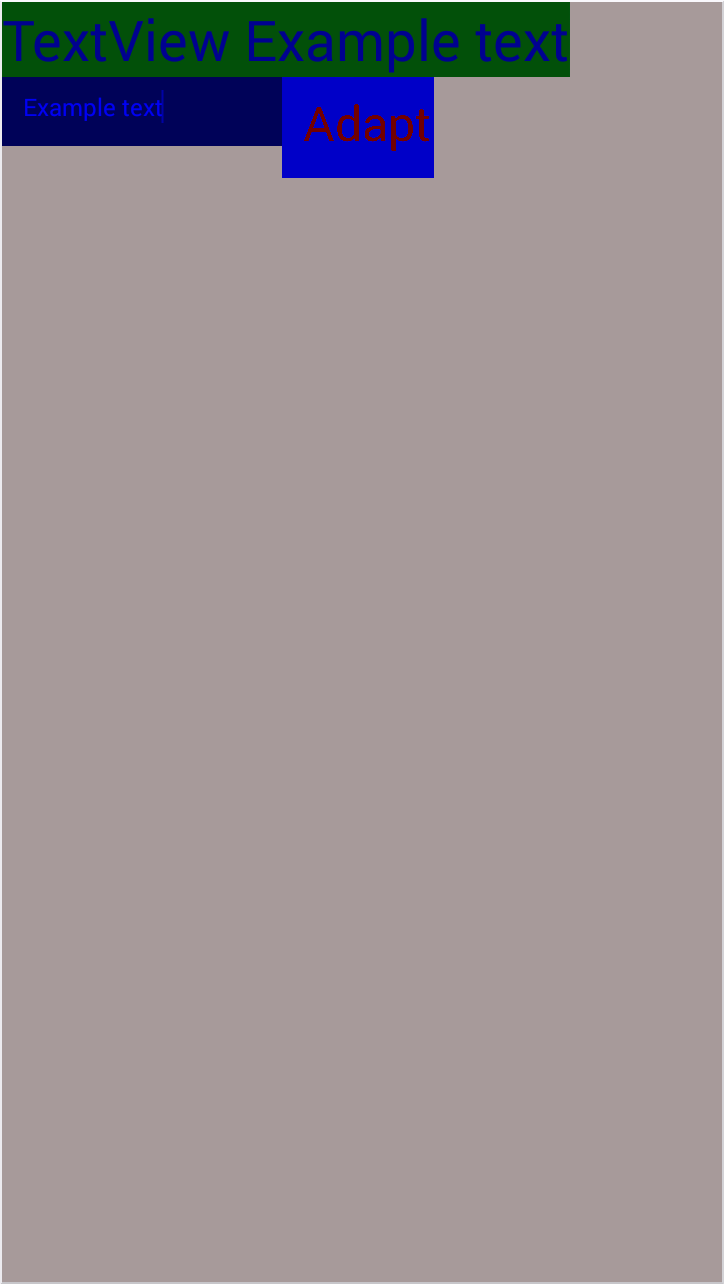
\includegraphics[width=0.25\textwidth]{adapted_layout.png}
\caption{The corresponding user interface considering the layout specified in
Listing~\ref{lst:adaptui_oncreate}.}
\label{fig:adapted_layout}
\end{figure}



\subsubsection{The knowledge editor \ac{api}}
\label{sec:knowledge_api}

